\section{Future work Notater}
\label{chp:futurework} 
\subparagraph{TA MED DETTE?}
As second important open problem is mapping our simple model to reality
in a more convincing way. In particular real work networks are far from ran-
dom: nodes want to talk to clusters of other nodes, and both friend ship and
link capacity is distributed according to a power law. Furthermore what mat-
ters in real world networks is not a short path merely existing, but also being
able to nd it within some reasonable time (social networks in particular are
navigable [7]). Modifying the friendship graph and link budgets to full those
requirements is an important next step
\subsection{Risk}
In our model we used an additive risk parameter, meaning that each connection to a non-insured node adds a fixed negative value $r$ to the node's utility. It is reasonable to assume that the probability of failure increases if a node accepts more and more non-insured nodes. However, whether the risk parameter increases according to an additive distribution is difficult to confirm. Hence the decision of using additive risk was take due to the simplicity of the function and the fact that we do not know for sure how the distribution actually looks like. The probability might as well be multiplicative, exponential or logarithmic. Although it is highly uncertain, we believe that the risk parameter will follow an exponential distribution similar to the one in Eq.(\ref{eq:distributionFunction}).

\begin{equation}
    F(x;\lambda)= 
\begin{cases}
    1-e^{-\lambda x} ,& \text{if } x \geq 0\\
   0,& \text{if }  x<0\\
    
    
\end{cases}
\label{eq:distributionFunction}
\end{equation}



\begin{figure}[h]
\centering
  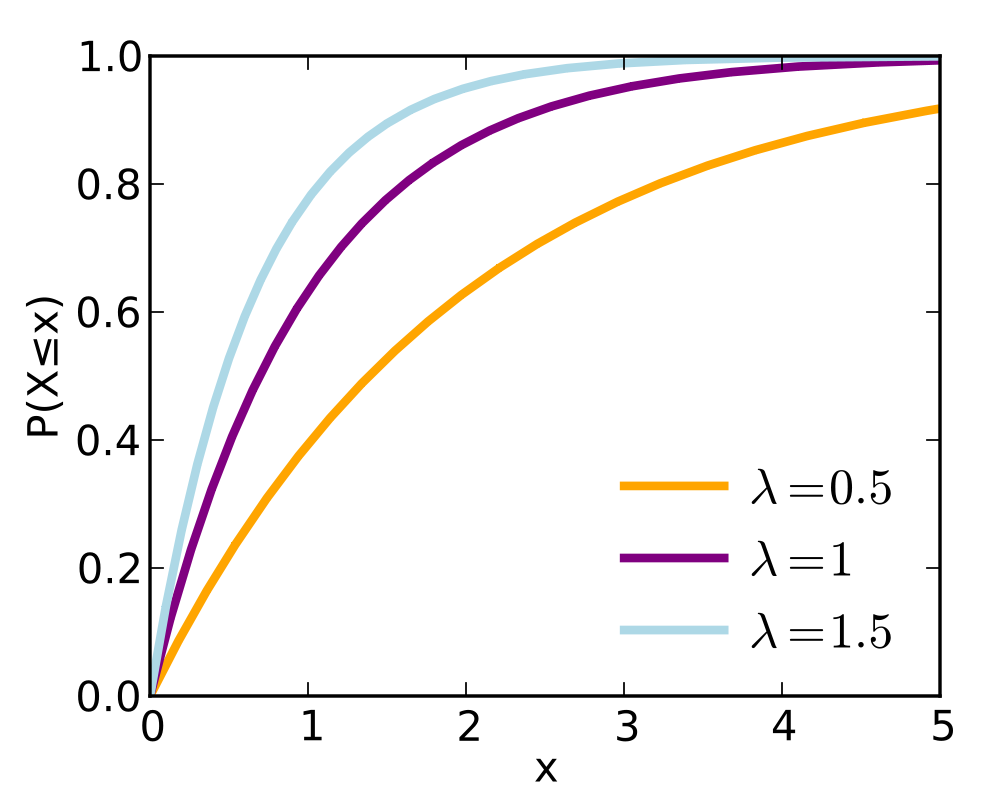
\includegraphics[width=0.5\linewidth]{../Figures/exponentialFunction.png}
  \caption{\label{fig:exponentialFunction} Figure showing the distribution of Eq.( \ref{eq:distributionFunction}). }
\end{figure}

When $\lambda$ have a value around 0.5, we get a curve \ref{fig:exponentialFunction} which captures how we believe the risk in a network will increase as more non-insured nodes are added. We believe that if one have a growing network consisting of insured nodes only, the first non-insured node added will contribute more risk than the consecutive non-insured nodes. When the 2.nd and 3.rd and so on, node are added there are already a probability that the network will be infected. It reasonable to believe that the overall risk wont increase additive, but at a lower rate. The risk added for each new non-insured node will decrease. Hence we believe that the accentual risk parameter will follow a exponential distribution. 

read more in the paper: Uncertainty in Interdependent Security Games

From this paper presents a description of how to measure risk within a local network. The idea is that for a cost $c$, you can protect yourself from threats outside your own LAN or corporation. This is analogous to purchase a firewall and anti-virus software. However, you can still be affected by threats from non-insured nodes inside your own local network. This means that as long as not every node is insured, the non-insured node will introduce a risk $q$ to the local network. $p$ reflects the probability of getting affected by a risk, and $q$ represents the likelihood of spreading it to others in the local network. The paper presents a swift model for measuring the risk in you local network.

\begin{equation}
    U_{i}= 
\begin{cases}
    -c + (1-q)^k ,& \text{if not buying insurance} \\
   (1-p)(1-q)^k,& \text{ifbuying insurance }  \\
    
    
\end{cases}
\label{eq:riskModel}
\end{equation}
 This model can be used to look at a the decision process of single node on whether to buy insurance or not. The paper presents certain conditions which creates scenarios where we end up with a network where either every node chooses to buy or every one chooses not to buy insured. 

If $c<p$ then everyone will buy insurance, since this is cheaper than the expected loss. The other equilibrium where no one buys insurance, occurs when the cost of insurance is higher that the likelihood that a player fails to protect him selves, assuming that also fails to protect. i.e. $c>p(1-q)^{1-n}$
 
Our model's ultimate goal is to end up with insurable topologies which are able to measure risk in networks with a mix of insured and non-insured nodes. Therefore we will not take the same approach towards handling the problem with internal risk, i.e always forcing the network to either consist of insured nodes or not not-insured nodes. Instead we want to transfer this risk to the insurance company. Each node will have the opportunity to purchase a link insurance, which compensate from any financial loss from a specific node. 